\documentclass[text06.tex]{subfiles}
\begin{document}
\chapter{音声合成と音声\ruby{認識}{にん|しき}}
\section{この章でやること}

この章では、Rapsberry Piに言葉を話させる方法と、言葉を聞き取らせる方法を学びます。
\ruby{機械}{き|かい}に言葉を話させることを「\ruby{音声合成}{おん|せい|ごう|せい}」、機械に言葉を聞き取らせることを「\ruby{音声認識}{おん|せい|にん|しき}」と呼びます。
この教材では、音声合成には\aruby{OpenJtalk}{オープンジェートーク}、音声認識には\aruby{Julius}{ジュリウス}というソフトウェアを使用します。
計算結果をRapsberry Piに話させたり、音声でLEDを点灯させたりしながら、Raspberry Piで音声を使った処理を実現してみましょう。

\subsection{教材を自分のフォルダに置こう}
まずは、今回利用する教材をコピーしましょう。
\nobreak/usr/local/share/ome にあるフォルダ 06 を自分のホームディレクトリに 07 という名前でコピーしてください。
\begin{lstlisting}[caption=ターミナルを使ったディレクトリのコピー,label=workfilecopy]
<#green#pi@raspberrypi#>:<#blue#~ $#> cp -r /usr/local/share/ome/06 ~/07/
<#green#pi@raspberrypi#>:<#blue#~ $#>
\end{lstlisting}

\newpage
\section{音声合成}
音声合成とは何でしょう。それは、人間の声を人工的に機械で作り出すことです。みなさんが目にするもので言えば、例えばアマゾン社が\ruby{開発}{かい|はつ}した図\ref{amazon_echo}の\aruby{Amazon Echo}{アマゾンエコー}という\ruby{製品}{せい|ひん}があります。

\begin{figure}[H]
\begin{center}
    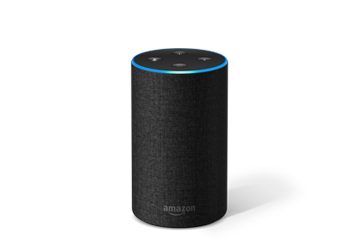
\includegraphics[width=.8\linewidth]{../../asset/image/amazon_echo.png}
    \caption{Amazon Echo\\（出典：Amazon.com, Inc）}
    \label{amazon_echo}
\end{center}
\end{figure}

Amazon Echoは音声アシスタントであるAlexaを通じて声を出して利用者の問いかけに\ruby{応答}{おう|とう}します。Amazon Echoから声が出るのは、中に人間が入っているわけではありません。読み上げたい文章があったとき、その文章に合った音声を作り、スピーカーから\ruby{鳴}{な}らしているのです。
今回は音声を合成するために、OpenJTalkと\ruby{呼}{よ}ばれる音声合成のためのソフトウェアを使います。OpenJTalkは、読み上げたい文章と、ひらがなごとの音（\ruby{厳密}{げん|みつ}にはもう少し多種の音）を入力し、\ruby{対応}{たい|おう}する音声ファイルを出力します（図\ref{OpenJTalkの入出力}）。

\begin{figure}[H]
\begin{center}
    \includesvg[width=.7\linewidth]{../../asset/image/text06-img011.svg}
    \caption{OpenJTalkの入出力}
    \label{OpenJTalkの入出力}
\end{center}
\end{figure}

\begin{tcolorbox}[title=\useOmetoi]
\begin{enumerate}
        \addquiz{音声合成とはなんですか。20字以内で説明してください。}
        \addquiz{音声合成をするにはパソコンに何を\ruby{準備}{じゅん|び}する必要がありますか。3つ挙げてください。}
\end{enumerate}
\end{tcolorbox}
\end{document}
